\documentclass{beamer}
\usepackage[utf8]{inputenc}

 
\usepackage[square,numbers]{natbib}
\usepackage{graphicx}
\usepackage{amsmath,amsfonts,amssymb,amsthm}
\usepackage{thmtools}
\usepackage{stmaryrd}
\usepackage{url}
\usepackage{array}
\usepackage{arydshln}
\usepackage{ifthen}
\usepackage{ifpdf}
\usepackage{verbatim}
\usepackage{listings}
\usepackage{mathpartir}

\usepackage{mathtools}
\DeclarePairedDelimiter\ceil{\lceil}{\rceil}
\DeclarePairedDelimiter\floor{\lfloor}{\rfloor}

\usepackage{appendix}

\usepackage{tikz}
\usepackage{multirow}

\newcommand{\forcenewline}{$\phantom{v}$\\}
\newcommand{\judgment}[2]{\paragraph{#1}\hspace{\stretch{1}}\fbox{$#2$}}

\newcommand{\update}[2]{[#1 \mapsto #2]}
\newcommand{\sem}[1]{\left\llbracket #1 \right\rrbracket}

% Math notation
\newcommand{\restrictfun}[1]{|_{#1}}
\newcommand{\parfun}{\rightharpoonup}
\newcommand{\finparfun}{\xrightharpoonup{\textit{\tiny{fin}}}}
\newcommand{\monnefun}{\xrightarrow{\textit{\tiny{mon, ne}}}}
\newcommand{\monfun}{\xrightarrow{\textit{\tiny{mon}}}}
\newcommand{\nefun}{\xrightarrow{\textit{\tiny{ne}}}}
\newcommand{\fun}{\rightarrow}
\newcommand{\defeq}{\stackrel{\textit{\tiny{def}}}{=}}
\newcommand{\nequal}[1][n]{\stackrel{\tiny{#1}}{=}}
\renewcommand{\nsim}[1][n]{\stackrel{\tiny{#1}}{\simeq}}

\newcommand\subsetsim{\mathrel{\ooalign{\raise.2ex\hbox{$\subset$}\cr
      \hidewidth\lower.8ex\hbox{\scalebox{0.9}{$\sim$}}\hidewidth\cr}}}
\newcommand\supsetsim{\mathrel{\ooalign{\raise.2ex\hbox{$\supset$}\cr
      \hidewidth\lower.8ex\hbox{\scalebox{0.9}{$\sim$}}\hidewidth\cr}}}
\newcommand{\nsubsim}[1][n]{\stackrel{\tiny{#1}}{\subsetsim}}
\newcommand{\nsupsim}[1][n]{\stackrel{\tiny{#1}}{\supsetsim}}

\newcommand{\nsubeq}[1][n]{\stackrel{\tiny{#1}}{\subseteq}}
\newcommand{\nsupeq}[1][n]{\stackrel{\tiny{#1}}{\supseteq}}

\newcommand{\union}{\mathbin{\cup}}
\DeclareMathOperator{\dom}{dom}
\newcommand{\blater}{\mathop{\blacktriangleright}}
\newcommand{\id}{\var{id}}
\newcommand{\undefined}{\mathit{undefined}}

\newcommand{\powerset}[1]{\mathcal{P}(#1)}

\newcommand{\false}{\mathit{false}}
\newcommand{\true}{\mathit{true}}


% cofes
\newcommand{\cofe}{c.o.f.e.}
\newcommand{\cofes}{\cofe{}'s}
\newcommand{\CatC}{\mathbb{C}}
\newcommand{\CatP}{\mathbb{P}}

% Comments
\newcommand\lau[1]{{\color{purple} \sf \footnotesize {LS: #1}}\\}
\newcommand\dominique[1]{{\color{purple} \sf \footnotesize {DD: #1}}\\}
\newcommand\lars[1]{{\color{purple} \sf \footnotesize {LB: #1}}\\}

% Variables
\newcommand{\var}[1]{\mathit{#1}}
\newcommand{\hs}{\var{ms}}
\newcommand{\ms}{\hs}
\newcommand{\hv}{\var{hv}}
\newcommand{\rv}{\var{rv}}
\newcommand{\lv}{\var{lv}}
\newcommand{\gl}{\var{g}}
\newcommand{\pc}{\mathit{pc}}
\newcommand{\pcreg}{\mathrm{pc}}
\newcommand{\addr}{\var{a}}
\newcommand{\offset}{\var{offset}}
\newcommand{\word}{\var{w}}
\newcommand{\start}{\var{base}}
\newcommand{\addrend}{\var{end}}
\newcommand{\pwlv}{\var{pwl}}
\newcommand{\mem}{\var{mem}}
\newcommand{\reg}{\var{reg}}
\newcommand{\heapseg}{\var{ms}}
\newcommand{\heap}{\var{mem}}
\newcommand{\perm}{\var{perm}}
\newcommand{\permp}{\var{permPair}}
\newcommand{\roll}{\var{roll}}
\newcommand{\instr}{\var{instr}}
\newcommand{\stdcap}[1][(\perm,\gl)]{\left(#1,\start,\addrend,\addr \right)}
\newcommand{\adv}{\var{adv}}
\newcommand{\msframe}{ms_\var{frame}}
\newcommand{\link}{\var{link}}
\newcommand{\stk}{\var{stk}}
\newcommand{\flag}{\var{flag}}
\newcommand{\nwl}{\var{nwl}}
\newcommand{\pwl}{\var{pwl}}
\newcommand{\sta}{\var{sta}}
\newcommand{\cnst}{\var{cnst}}
\newcommand{\olf}{\var{offsetLinkFlag}}
\newcommand{\prp}{\var{prp}}

% Memory projections
\newcommand{\plainproj}[1]{\mathrm{#1}}
\newcommand{\memheap}[1][\Phi]{#1.\plainproj{mem}}
\newcommand{\memreg}[1][\Phi]{#1.\plainproj{reg}}

\newcommand{\updateHeap}[3][\Phi]{#1\update{\plainproj{mem}.#2}{#3}}
\newcommand{\updateReg}[3][\Phi]{#1\update{\plainproj{reg}.#2}{#3}}

% Configuration end states
\newcommand{\failed}{\textsl{failed}}
\newcommand{\halted}{\textsl{halted}}

% Functions
\newcommand{\plainfun}[2]{
  \ifthenelse{\equal{#2}{}}
  {\mathit{#1}}
  {\mathit{#1}(#2)}
}
\newcommand{\decode}{\plainfun{decode}{}}
\newcommand{\encode}{\plainfun{encode}{}}
\newcommand{\encodePerm}{\mathit{encodePerm}}
\newcommand{\encodePermPair}{\plainfun{encodePermPair}{}}
\newcommand{\encodeLoc}{\mathit{encodeLoc}{}}
\newcommand{\decodePermPair}{\plainfun{decodePermPair}}
\newcommand{\decodePerm}[1]{\plainfun{decodePerm}{#1}}
\newcommand{\updatePcPerm}[1]{\plainfun{updatePcPerm}{#1}}

\newcommand{\executeAllowed}[1]{\plainfun{executeAllowed}{#1}}
\newcommand{\nonZero}[1]{\plainfun{nonZero}{#1}}
\newcommand{\readAllowed}[1]{\plainfun{readAllowed}{#1}}
\newcommand{\writeAllowed}[1]{\plainfun{writeAllowed}{#1}}
\newcommand{\withinBounds}[1]{\plainfun{withinBounds}{#1}}
\newcommand{\stdUpdatePc}[1]{\plainfun{updatePc}{#1}}

\newcommand{\readCond}[1]{\plainfun{readCondition}{#1}}
\newcommand{\writeCond}[1]{\plainfun{writeCondition}{#1}}
\newcommand{\execCond}[1]{\plainfun{executeCondition}{#1}}
\newcommand{\entryCond}[1]{\plainfun{enterCondition}{#1}}

\newcommand{\revokeTemp}[1]{\plainfun{revokeTemp}{#1}}
\newcommand{\erase}[2]{\floor*{#1}_{\{#2\}}}
\newcommand{\activeReg}[1]{\plainfun{active}{#1}}

% World operations
\newcommand{\future}{\mathbin{\sqsupseteq}}
\newcommand{\futurewk}{\mathbin{\sqsupseteq}^{\var{pub}}}
\newcommand{\futurestr}{\mathbin{\sqsupseteq}^{\var{priv}}}
\newcommand{\heapSat}[3][\heap]{#1 :_{#2} #3}
\newcommand{\memSat}[3][n]{\heapSat[#2]{#1}{#3}}
\newcommand{\memSatPar}[4][n]{\heapSat[#2]{#1 , #4}{#3}}

\newcommand{\monwknefun}{\xrightarrow[\text{\tiny{$\futurewk$}}]{\textit{\tiny{mon, ne}}}}
\newcommand{\monwkfun}{\xrightarrow[\text{\tiny{$\futurewk$}}]{\textit{\tiny{mon}}}}
\newcommand{\monstrnefun}{\xrightarrow[\text{\tiny{$\futurestr$}}]{\textit{\tiny{mon, ne}}}}


% Assembly labels
\newcommand{\codelabel}[1]{\mathit{#1}}
\newcommand{\init}{\codelabel{init}}
\newcommand{\malloc}{\codelabel{malloc}}
\newcommand{\counter}{\codelabel{counter}}
\newcommand{\iocap}{\codelabel{iocap}}

% Type(s)
\newcommand{\type}[1]{\mathrm{#1}}
\newcommand{\asmType}{\plaindom{AsmType}}


% Domains
\newcommand{\plaindom}[1]{\mathrm{#1}}
\newcommand{\Caps}{\plaindom{Cap}}
\newcommand{\Words}{\plaindom{Word}}
\newcommand{\Addrs}{\plaindom{Addr}}
\newcommand{\ExecConfs}{\plaindom{ExecConf}}
\newcommand{\RegName}{\plaindom{RegisterName}}
\newcommand{\Regs}{\plaindom{Reg}}
\newcommand{\Heaps}{\plaindom{Mem}}
\newcommand{\Mems}{\Heaps}
\newcommand{\HeapSegments}{\plaindom{MemSegment}}
\newcommand{\MemSegments}{\HeapSegments}
\newcommand{\Confs}{\plaindom{Conf}}
\newcommand{\Instrs}{\plaindom{Instructions}}
\newcommand{\nats}{\mathbb{N}}
\newcommand{\ints}{\mathbb{Z}}
\newcommand{\Perms}{\plaindom{Perm}}
\newcommand{\Globals}{\plaindom{Global}}

\newcommand{\Rel}{\plaindom{Rel}}
\newcommand{\States}{\plaindom{State}}
\newcommand{\RegionNames}{\plaindom{RegionName}}
\newcommand{\Regions}{\plaindom{Region}}
\newcommand{\Reg}{\plaindom{Reg}}
\newcommand{\Worlds}{\plaindom{World}}
\newcommand{\Wor}{\plaindom{Wor}}
\newcommand{\Worwk}{\Wor_{\futurewk}}
\newcommand{\Worstr}{\Wor_{\futurestr}}
\newcommand{\xiwk}{\xi_{\var{wk}}}
\newcommand{\xistr}{\xi_{\var{str}}}
\newcommand{\StorePred}{\plaindom{MemSegPred}}
\newcommand{\UPred}[1]{\plaindom{Pred}(#1)}
\newcommand{\DCPred}[1]{\plaindom{P}^\downarrow(#1)}

\newcommand{\Views}{\plaindom{View}}

% LR
\newcommand{\intr}[2]{\mathcal{#1}}
\newcommand{\valueintr}[1]{\intr{V}{#1}}
\newcommand{\exprintr}[1]{\intr{E}{#1}}
\newcommand{\contintr}[1]{\intr{K}{#1}}
\newcommand{\regintr}[1]{\intr{R}{#1}}
\newcommand{\stdvr}{\valueintr{\asmType}}
\newcommand{\stder}{\exprintr{\asmType}}
\newcommand{\stdrr}{\regintr{\asmType}}
\newcommand{\stdkr}{\contintr{\asmType}}
\newcommand{\observations}{\mathcal{O}}
\newcommand{\npair}[2][n]{\left(#1,#2 \right)}

% Reference register/memory
\newcommand{\refreg}[1]{#1}
\newcommand{\refheap}[1]{#1}

% Instructions
% No arguments
\newcommand{\zinstr}[1]{\mathtt{#1}}
\newcommand{\fail}{\zinstr{fail}}
\newcommand{\halt}{\zinstr{halt}}
% One argument
\newcommand{\oneinstr}[2]{\zinstr{#1} \; #2}
\newcommand{\jmp}[1]{\oneinstr{jmp}{#1}}
% Two arguments
\newcommand{\twoinstr}[3]{\zinstr{#1} \; #2 \; #3}
\newcommand{\restricttwo}[2]{\twoinstr{restrict}{#1}{#2}}
\newcommand{\jnz}[2]{\twoinstr{jnz}{#1}{#2}}
\newcommand{\isptr}[2]{\twoinstr{isptr}{#1}{#2}}
\newcommand{\geta}[2]{\twoinstr{geta}{#1}{#2}}
\newcommand{\getb}[2]{\twoinstr{getb}{#1}{#2}}
\newcommand{\gete}[2]{\twoinstr{gete}{#1}{#2}}
\newcommand{\getp}[2]{\twoinstr{getp}{#1}{#2}}
\newcommand{\getl}[2]{\twoinstr{getl}{#1}{#2}}
\newcommand{\move}[2]{\twoinstr{move}{#1}{#2}}
\newcommand{\store}[2]{\twoinstr{store}{#1}{#2}}
\newcommand{\load}[2]{\twoinstr{load}{#1}{#2}}
\newcommand{\lea}[2]{\twoinstr{lea}{#1}{#2}}
% Three arguments
\newcommand{\threeinstr}[4]{\zinstr{#1} \; #2 \; #3 \; #4}
\newcommand{\restrict}[3]{\threeinstr{restrict}{#1}{#2}{#3}}
\newcommand{\subseg}[3]{\threeinstr{subseg}{#1}{#2}{#3}}
\newcommand{\plus}[3]{\threeinstr{plus}{#1}{#2}{#3}}

% Permissions
\newcommand{\plainperm}[1]{\mathrm{#1}}
\newcommand{\noperm}{\plainperm{o}}
\newcommand{\readonly}{\plainperm{ro}}
\newcommand{\readwrite}{\plainperm{rw}}
\newcommand{\exec}{\plainperm{rx}}
\newcommand{\entry}{\plainperm{e}}
\newcommand{\rwx}{\plainperm{rwx}}
% PWL permissions
\newcommand{\readwritel}{\plainperm{rwl}}
\newcommand{\rwl}{\readwritel}
\newcommand{\rwlx}{\plainperm{rwlx}}

% Global/local
\newcommand{\local}{\plainperm{local}}
\newcommand{\glob}{\plainperm{global}}

\newcommand{\localityReg}{\var{localityReg}}
\newcommand{\localReg}{\var{localReg}}
\newcommand{\globalReg}{\var{globalReg}}

% Views
\newcommand{\plainview}[1]{\mathrm{#1}}
\newcommand{\perma}{\plainview{perm}}
\newcommand{\temp}{\plainview{temp}}
\newcommand{\revoked}{\plainview{revoked}}

% OP sem
\newcommand{\diverge}[1][n]{\not\Downarrow_{#1}}
\newcommand{\step}[1][]{\rightarrow_{#1}}

\lstset{basicstyle=\footnotesize\ttfamily,breaklines=true}

\AtBeginSection[]
{
  \begin{frame}<beamer>
    \frametitle{Road map}
    \tableofcontents[currentsection]
  \end{frame}
}

\newsavebox{\locstatebox}
\newsavebox{\tdbox}
\newsavebox{\continuationbox}
\newsavebox{\awkwardex}

\title{Tales of Belgium: Reasoning about Capability Machines using Logical Relations}
\author{Lau Skorstengaard}
\institute{Aarhus University}
\date{Aarhus University, December 2016}
\begin{document}
\frame{\titlepage}

\frame{
  \frametitle{Road map}
  \tableofcontents
}

\begin{frame}
  \frametitle{Leuven}
  \begin{figure}
    \centering
    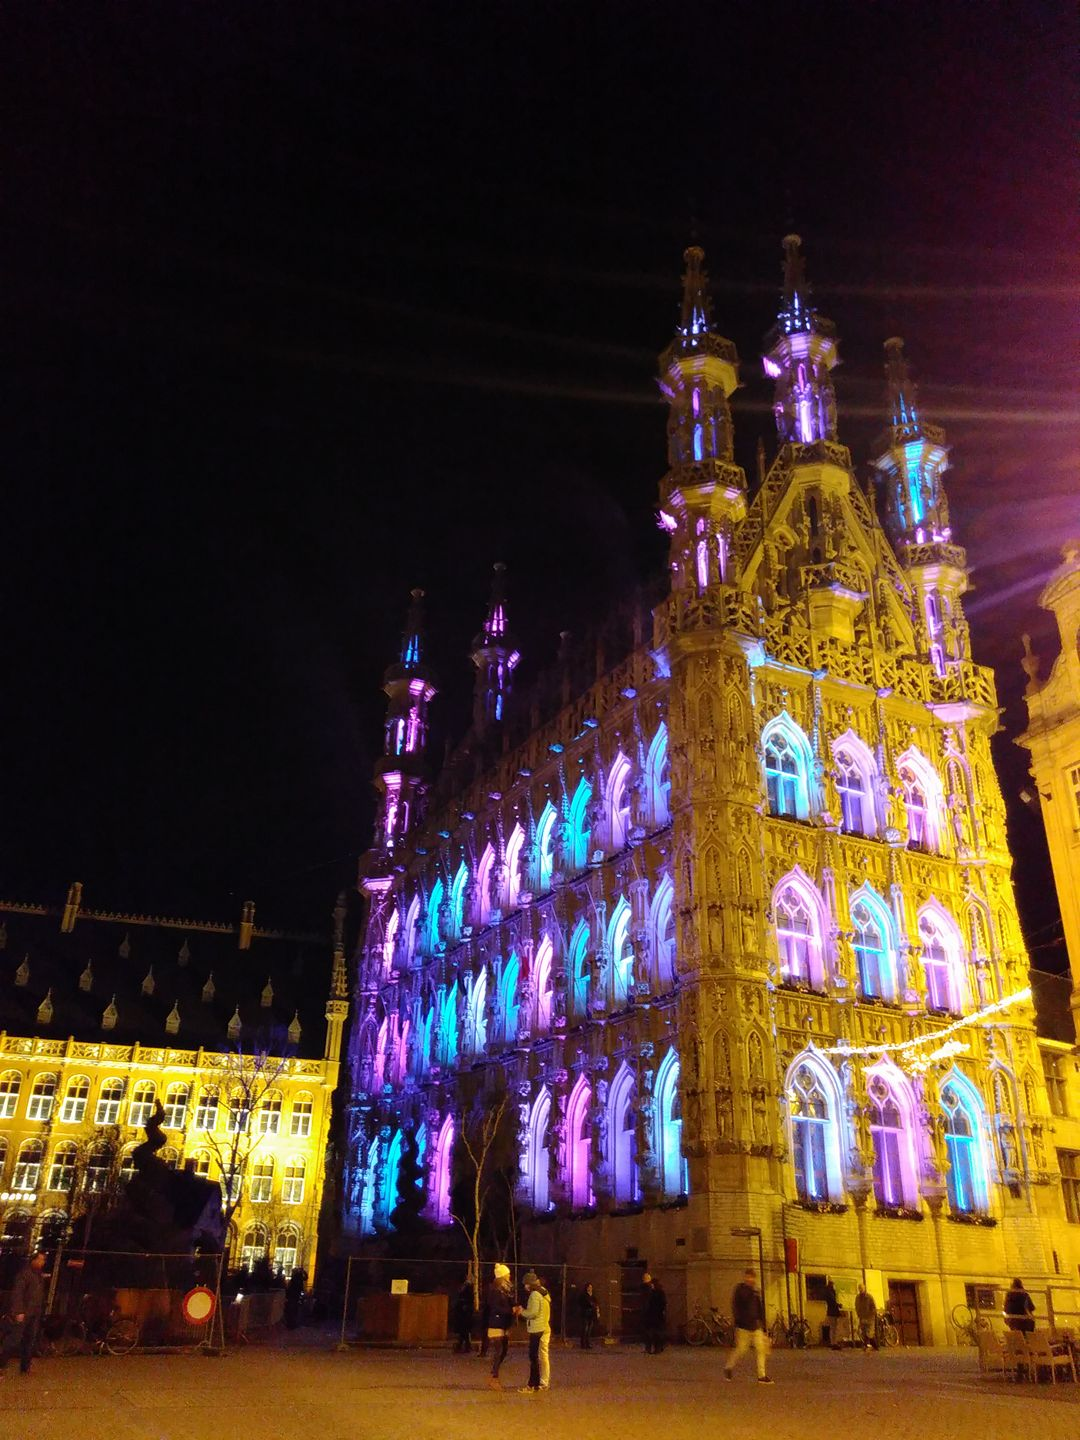
\includegraphics[scale=0.15]{leu1}
\end{figure}
\end{frame}
\begin{frame}
  \frametitle{Leuven}
\onslide<2->
  \begin{figure}
    \centering
    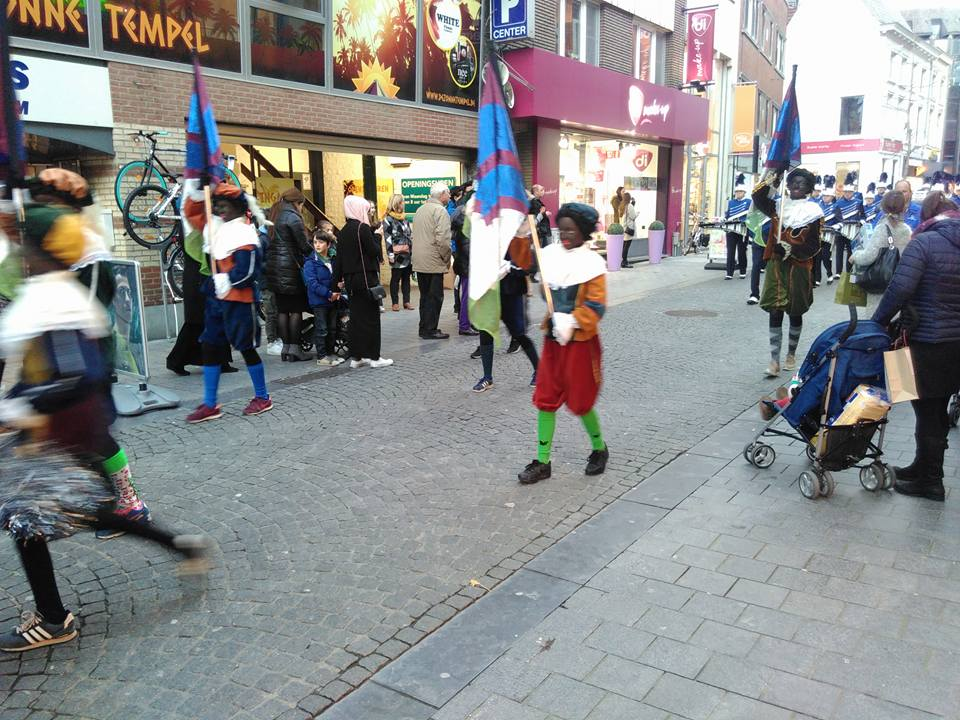
\includegraphics[scale=0.3]{leu2}
\end{figure}
\end{frame}

\section{Capability Machine}
\begin{frame}
  \frametitle{ Why should I care about capability machines? }
  \textbf{Current low-level protection mechanisms}
  \begin{itemize}
  \item Coarse-grained compartmentalisation 
  \item Expensive context switches 
  \item Well suited for high-level applications
  \item Does not scale well
  \item E.g., virtual memory
  \end{itemize}
\end{frame}

\begin{frame}
  \frametitle{ Why should I care about capability machines? }
  \textbf{Capability machines}
  \begin{itemize}
  \item Fine-grained compartmentalisation
  \item Cheap compartments
  \item Fine-grained sharing
  \item Well suited for applications with need for many compartments
  \end{itemize}
\end{frame}

%\subsection{Simple Capability Machine}
\frame{
  \frametitle{ Capabilities }
  What is a capability? \pause
  \begin{itemize}
  \item<2-> \emph{Unforgeable} token of authority 
  \end{itemize} \pause
  What is a capability in a capability machine?
  \begin{itemize}
  \item<4-> Unforgeable pointer
    % In a normal machine, you can use an integer as a pointer (not unforgeable)
    % No way to generate capabilities.
    % System enforces this (tagged).
  \item<5-> Range of memory
    % Authority over range of memory, may be one cell, doesn't have to be.
  \item<6-> Permission
    % Kind of authority.
    % What can this capability be used for.
  \end{itemize}
\uncover<4-6>{
  \begin{figure}
    \centering
    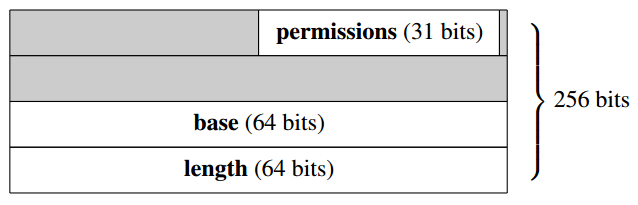
\includegraphics[width=0.8\textwidth]{chericap}
    \caption{CHERI capability \cite{Woodruff:2014:CCM:2665671.2665740}}
    \label{fig:chericap}
  \end{figure}
}
}

\frame{
\frametitle{Capability permissions}
\begin{itemize}
\item Read
\item Write
\item Execute
\item<2-> Enter
%Inspired by the M-Machine
  \begin{itemize}
  \item<3-> When jumped to, it becomes a read and execute capability
  \item<3-> Cannot be used in any other way
  \item<4-> Used by distrusting pieces of code to cross security boundaries
  \item<5-> Modularisation
  \end{itemize}
\end{itemize}
}

\frame{
\frametitle{Capability machine instructions}
\begin{itemize}
\item<1-> Same instructions as in a normal low-level machine
  \begin{itemize}
  \item<2-> \texttt{\emph<3>{jmp}}, \texttt{\emph<3>{jnz}}, \texttt{move}, \texttt{plus}, \texttt{\emph<3>{load}}, \texttt{\emph<3>{store}}
  \item<3-> Instructions may require capability with certain permission.
    %jmp has to be to an execute capability
    %load has to be through a read capability
    %store has to be through a write capability
  \end{itemize}
\item<4-> Capability manipulation instructions
  \begin{itemize}
  \item<5-> \texttt{lea}, \texttt{restrict}, \texttt{subseg} 
  \item<6-> No instruction generates new capability
  \item<7-> Manipulation of capabilities cannot result in authority amplification
  \end{itemize}
\end{itemize}
}

\frame{
\frametitle{Capability machine overview}
\begin{itemize}[<+->]
\item Capabilities 
  \begin{itemize}
  \item Permissions
  \item Range of authority
  \end{itemize}
\item Capability aware instructions
\item Memory and registers
  \begin{itemize}
  \item Can contain data and capabilities
  \item Capabilities tagged
    %Capabilities can be distinguished from data using tagging (file or bit in cap).
  \end{itemize}
\end{itemize}
}

%\subsection{Capability Machine with Local Capabilities}
\begin{frame}
  \frametitle{ Simple capability machine limitations }
  \begin{itemize}[<+->]
  \item No revocation of capabilities
  \item Simulating revocation of enter capabilities:
    \begin{itemize}
    \item On jump overwrite first address with fail instruction
    \item Subsequent jumps fail
    \end{itemize}
  \item Issues:
    \begin{itemize}
    \item Memory leak
    \item Does not scale to other types of permissions  
    \end{itemize}
  \end{itemize}
\end{frame}

\begin{frame}
  \frametitle{ Local capabilities }
  \begin{itemize}[<+->]
  \item Idea: New type of capability that cannot be stored when ``crossing security boundaries''
  \item Capabilities get two new fields:
    \begin{itemize}
    \item Local/(global)
    \item Permit write local (pwl)
    \end{itemize}
  \item Only pwl-capabilities can write local capabilities.
  \item Gives simple temporal revocation, but 
    \begin{itemize}
    \item requires no global pwl-capabilities
    \item enforcement depends on programming discipline.
    \end{itemize}
  \end{itemize}
\end{frame}


\begin{frame}
  \frametitle{Brussels}
  \begin{figure}
    \centering
    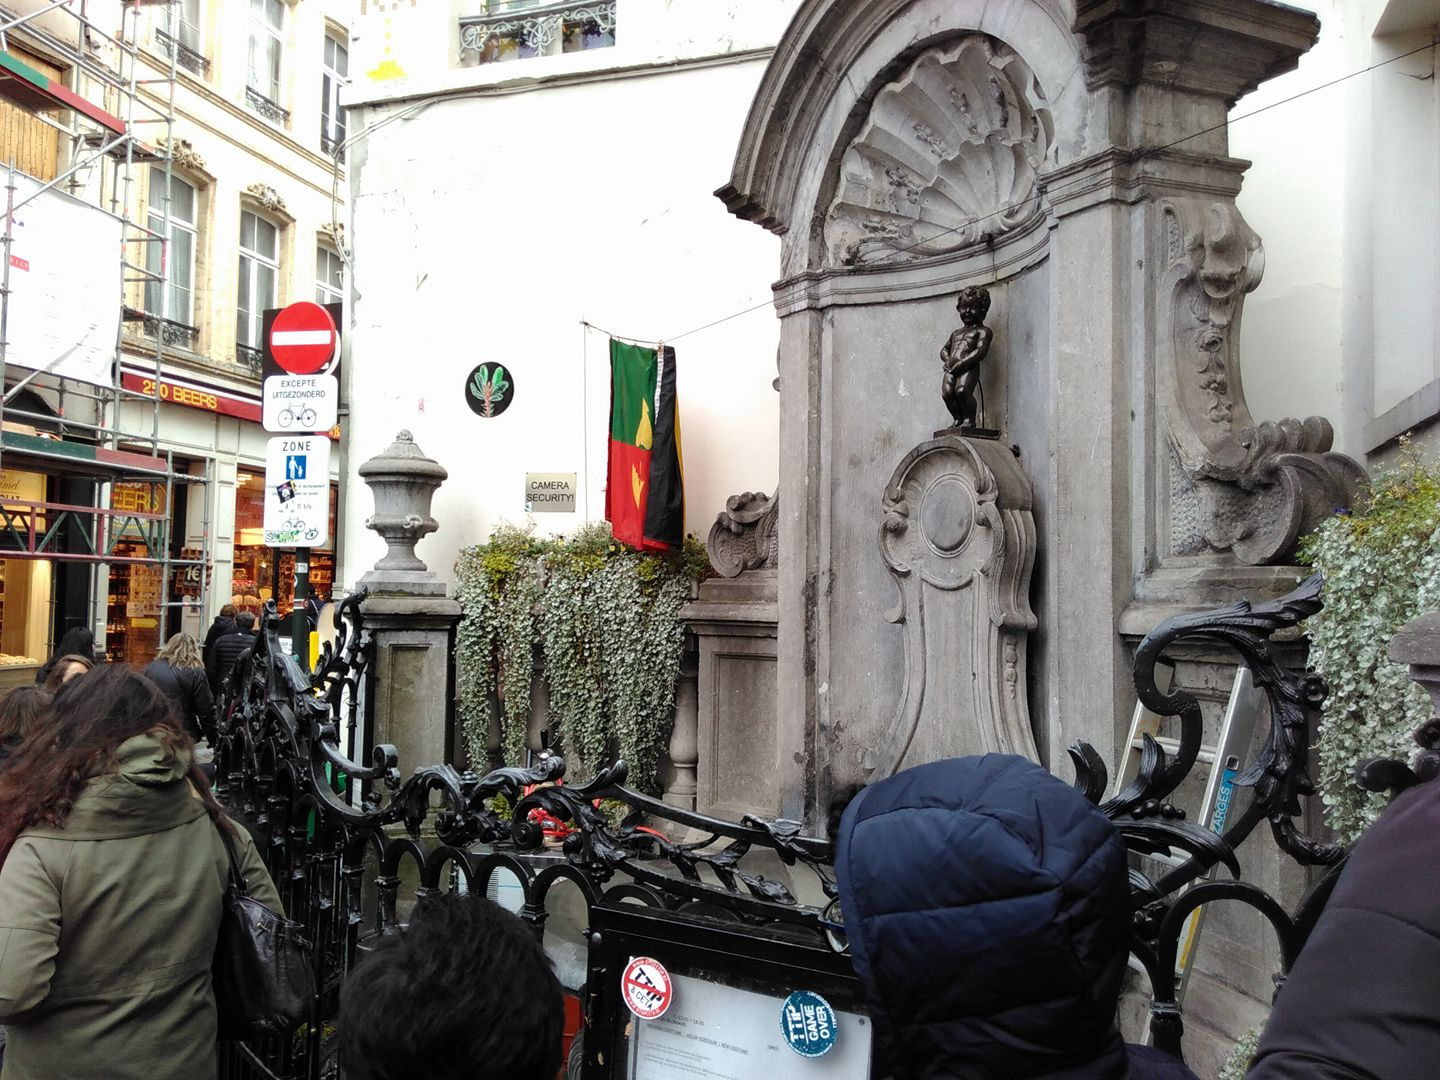
\includegraphics[scale=0.2]{bru}
\end{figure}
\end{frame}

\section{Formalisation}
\frame{
  \frametitle{Formalisation - Permissions}
  \textbf{Permissions}
  \begin{itemize}
  \item To simplify matters, we only allow certain combinations of permissions
  \item<2-> No permissions, \uncover<3->{read only,} \uncover<4->{read-write,} \uncover<8->{read-'write-local'} \uncover<5->{read-execute,} \uncover<6->{enter,} \uncover<7->{read-write-execute,} \uncover<8->{read-'write-local'-execute}
  \end{itemize}

  \[
    \Perms \defeq \{ \uncover<2->{\noperm,} \uncover<3->{\readonly,} \uncover<4->{\readwrite,} \uncover<8->{\rwl,} \uncover<5->{\exec,} \uncover<6->{\entry,} \uncover<7->{\rwx,} \uncover<8->{\rwlx}\}
  \]
}

\frame{
  \frametitle{Formalisation - Permissions}
  \textbf{Permissions ordering}
\begin{figure}[!h]
  \centering
  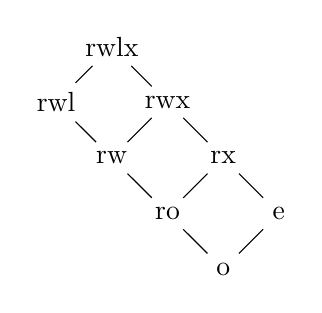
\begin{tikzpicture}[main node/.style={}]
    \node[main node] (7) {$\rwlx$};
    \node[main node] (8) [below left of=7] {$\readwritel$};
    \node[main node] (1) [below right of=7] {$\rwx$};
    \node[main node] (2) [below right of=1] {$\exec$};
    \node[main node] (3) [below right of=2] {$\entry$};
    \node[main node] (4) [below left of=1] {$\readwrite$};
    \node[main node] (5) [below right of=4] {$\readonly$};
    \node[main node] (6) [below right of=5] {$\noperm$};

    \path[every node/.style={font=\sffamily\small}]
    (7) edge (8)
    (7) edge (1)
    (8) edge (4)
    (1) edge (2)
    (2) edge (3)
    (2) edge (5)
    (3) edge (6)
    (1) edge (4)
    (4) edge (5)
    (5) edge (6);
  \end{tikzpicture}

  \caption{Permission hierarchy}
  \label{fig:perm-hier}
\end{figure}
}

\begin{frame}
\frametitle{ Formalisation - Locality }
\textbf{Locality}
\[
  \Globals ::= \{\glob, \local \}
\]
\textbf{Locality ordering}
\begin{figure}[!h]
  \centering
  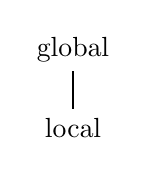
\begin{tikzpicture}[main node/.style={}]
    \node[main node] (1) {$\glob$};
    \node[main node] (2) [below of=1] {$\local$};

    \path[every node/.style={font=\sffamily\small}]
    (1) edge (2);
  \end{tikzpicture}
  \caption{Locality hierarchy}
  \label{fig:glob-hier}
\end{figure}
\end{frame}


\frame{
  \frametitle{Formalisation - Capabilities}

  \textbf{Capability}
  \begin{itemize}
  \item<2-> Permission and locality
  \item<4-> Range of authority
  \item<7-> Pointer
  \end{itemize}

  \[
    \uncover<5->{\Addrs \defeq \nats}
  \]

  \[
    \Caps \defeq \uncover<3->{(\Perms \times \Globals)} \uncover<6->{\times \Addrs \times \Addrs} \uncover<8->{\times \Addrs}
  \]
  \uncover<9->{
    Example: $((\entry,\local), 30, 42, 30)$
  }
}

\frame{
  \frametitle{Formalisation - Words and register file}
  \textbf{Words}
  \begin{itemize}
  \item<2-> Capability
  \item<4-> Data (and instructions)
  \item<6-> In the real machine capabilities are tagged 
  \end{itemize}
  \[
    \Words \defeq \uncover<3->{\Caps} \uncover<5->{+ \ints}
  \]
  \uncover<7->{
    \textbf{Register file}
    \begin{itemize}
    \item<8-> Assume finite set of registers $\RegName \ni \pcreg$ 
    \end{itemize}
    \[
      \Regs \defeq \uncover<9->{\RegName \rightarrow \Words}
    \]
  }
}

\frame{
  \frametitle{Formalisation - Memory and configurations}
  \textbf{Memory}
  \begin{itemize}
  \item<2-> Map from $\Addrs$ to $\Words$
    % Example of abstraction
    % Notice there are infinitely many addresses, so the heap is infinite!
    % We only allow finite use of it.
    % This is to avoid dealing with "out of memory" 
  \end{itemize}
  \[
    \Heaps \defeq \uncover<2->{ \Addrs \rightarrow \Words }
  \]

\uncover<3->{
  \textbf{Configuration}
  \begin{itemize}
  \item<4-> Executable configuration
  \item<6-> Successfully halted configuration
  \item<8-> Failed configuration
  \end{itemize}
  \[
    \Confs \defeq\uncover<5->{\Regs \times \Heaps} 
                 \uncover<8->{ + \{ \failed \} }
                 \uncover<7->{ + \{\halted\} \times \Heaps}
  \]
}
}

\begin{frame}
  \frametitle{Formalisation - Instructions}
  \textbf{Syntax}
  \begin{itemize}
  \item<3-> The normal instructions
  \item<5-> The capability manipulation instructions
  \item<7-> Instructions to stop the machine
  \end{itemize}
  $$\begin{array}{rcl}
   \uncover<2->{\rv     &::=& n \mid r }\\
   \Instrs &::=& 
\uncover<4->{
                 \jmp{r} \mid \jnz{r}{\rv} \mid \move{r}{\rv} \mid \\
           &   & \load{r}{r} \mid \store{r}{r} \mid \plus{r}{\rv}{\rv}
} 
\uncover<6->{
                 \mid\\
           &   & \lea{r}{\rv} \mid \restrict{r}{r}{\rv} \mid  \\
           &   & \subseg{r}{\rv}{\rv} \mid \\
           &   & \getp{r}{r} \mid \getl{r}{r} \mid \getb{r}{r} \mid \\
           &   & \gete{r}{r} \mid \geta{r}{r}
}
\uncover<8->{
\mid \fail \mid \halt}

  \end{array}$$

\end{frame}

\begin{frame}
  \frametitle{Formalisation - Operational Semantics (1)}
  \textbf{Execution relation}
  \[
    \step \subseteq (\Regs \times \Heaps) \times \Confs
  \]

  \begin{mathpar}
\uncover<2->{
    \inferrule{ \uncover<3->{\memreg(\pcreg) = \stdcap[(\perm,\gl)]} \\ 
                \uncover<4->{\start \leq \addr \leq \addrend} \\
                \uncover<5->{\perm \in \{ \exec,\rwx,\rwlx \} } }
              { \var{executionAllowed}(\Phi) }
}
    \and
\uncover<6->{
   \inferrule{ \neg \var{executionAllowed}(\Phi) }
             { \Phi \step \uncover<7->{ \failed } }
}
    \and
\uncover<8->{
    \inferrule{ \var{executionAllowed}(\Phi) \\
                \uncover<9->{i = \memheap(a)}}
              { \Phi \step \uncover<10->{\llbracket} \uncover<9->{i} \uncover<10->{\rrbracket(\Phi)} }
} 
  \end{mathpar}
\end{frame}

\begin{frame}
  \frametitle{Formalisation - Operational Semantics (2)}
    \begin{mathpar}
      \inferrule{
        \only<2->{\var{w} = \memreg(r_2)}
        \only<1>{\phantom{\var{w} = \memreg(r_2)}} \\
%
        \only<3->{\memreg(r_1) = \stdcap}
        \only<1-2>{\phantom{\memreg(r_1) = \stdcap}}\\
%
        \only<4->{\perm \in \{\readwrite, \rwl, \rwx, \rwlx \}} 
        \only<1-3>{\phantom{\perm \in \{\readwrite, \rwl, \rwx, \rwlx \} }} \\
%
        \only<5->{\start \leq \addr \leq \addrend} 
        \only<1-4>{\phantom{\start \leq \addr \leq \addrend}}\\
%
        \only<6->{w=((\_,\local),\_,\_,\_) \only<7->{\Rightarrow \perm \in \{\rwl,\rwlx \}} }
        \only<1-6>{\phantom{\only<1-5>{w=((\_,\local),\_,\_,\_) }\Rightarrow \perm \in \{\rwl,\rwlx \}} }
}
      {\sem{\store{\refreg{r_1}}{\refheap{r_2}}}(\Phi) = 
        \only<8->{\var{updatePc}(}
        \only<1-7>{\phantom{\var{updatePc}(}}
          \only<2->{\updateHeap{\only<2>{r_1}\only<3->{\addr}}{\var{w}}}
          \only<1>{\phantom{\updateHeap{\only<2>{r_1}\only<3->{\addr}}{\var{w}}}}
        \only<8->{)}
        \only<1-7>{\phantom{)}} 
}
    \and
\uncover<13->{
      \inferrule{
        \only<14->{\memreg(r_2) = \stdcap[\var{permPair}]}
        \only<1-13>{\phantom{\memreg(r_2) = \stdcap[\var{permPair}]}} \\
        \only<15->{\var{newPermPair} = \decodePermPair{\Phi,r_3}}
        \only<1-14>{\phantom{\var{newPermPair} = \decodePermPair{\Phi,r_3}}}\\
        \only<16->{\var{newPermPair} \sqsubseteq \var{permPair}}
        \only<1-15>{\phantom{\var{newPermPair} \sqsubseteq \var{permPair}}}\\
        \only<17->{c = (\var{newPermPair},\start,\addrend,\addr) }
        \only<1-16>{\phantom{c = (\var{newPermPair},\start,\addrend,\addr) }}
      }
      { 
        \sem{\restrict{\refreg{r_1}}{r_2}{r_3}} =
        \only<18->{ \var{updatePc}( }
        \only<1-17>{\phantom{\var{updatePc}( } }
          \updateReg{r_1}{\var{c}}
        \only<18->{  )}
        \only<1-17>{\phantom{  )}}
      }
}
\and
\uncover<9->{
      \inferrule{ 
        \only<10->{\memreg(\pcreg) = \stdcap}
        \only<1-9>{\phantom{\memreg(\pcreg) = \stdcap}} \\
        \only<11->{\var{newPc} = (\perm,\start,\addrend,\addr + 1)}
        \only<1-10>{\phantom{\var{newPc} = (\perm,\start,\addrend,\addr + 1)}}
      }
      { \stdUpdatePc{\Phi} = \updateReg{\pcreg}{\only<12->{\var{newPc}} \only<1-11>{\phantom{\var{newPc}}}} 
      }
}
    \end{mathpar}
\end{frame}

\begin{frame}{Formalisation - Operational Semantics (3)}
  \begin{itemize}[<+->]
  \item Need a $\failed$ case for each of the rules
  \item The operational semantics of the remaining instructions is defined in a similar fashion
  \end{itemize}
\end{frame}

\begin{lrbox}{\awkwardex}
\begin{lstlisting}
g = fun _ => 
      let x = 0 in
      fun f =>
        x := 0;
        f();
        x := 1;
        f();
        assert(x == 1)
\end{lstlisting}
\end{lrbox}

\begin{frame}
  \frametitle{Antwerp}
  \begin{figure}
    \centering
    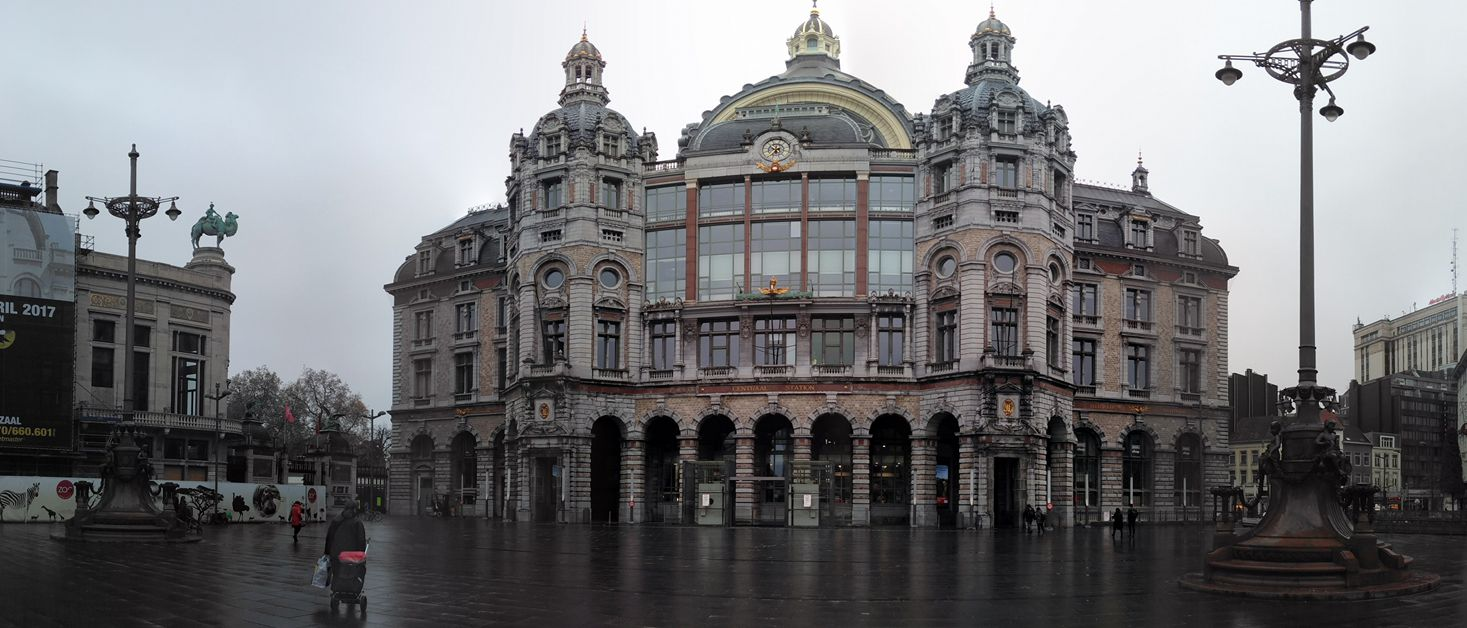
\includegraphics[scale=0.2]{ant}
\end{figure}
\end{frame}

\section{Example, Macros, and Stack Discipline}

\begin{frame}
  \frametitle{The ``awkward'' example }
      \usebox{\awkwardex}      
      \begin{itemize}
      \item<2-> Show for any reasonable \texttt{adv} that the assertion never fails for \texttt{adv(g)}.
      \item<3-> Need to define some macros to make a readable translation.
      \end{itemize}
\end{frame}

\begin{frame}
  \frametitle{Macros}
  \begin{itemize}[<+->]
  \item $\mathtt{crtcls} \;[(x_1,r_1),\dots, (x_n,r_n)] \; r$ 
    \begin{itemize}
    \item creates closure
    \item $x_1, \dots, x_n$ available in program
    \item $r$ capability for program
    \end{itemize}
  \item $\mathtt{assert} \; \rv_1 \; \rv_2$
    \begin{itemize}
    \item check whether $\rv_1$ and $\rv_2$ contains the same value
      \begin{itemize}
      \item if so: continue execution
      \item if not: set assertion flag and halt
      \end{itemize}
    \end{itemize}
  \item $\mathtt{malloc} \; r \; n$ 
    \begin{itemize}
    \item allocates a \emph{fresh} piece of memory of size $n$
    \item leaves a $\glob$ capability with $\rwx$ permission in register $r$
    \end{itemize}
  \end{itemize}
\end{frame}

\begin{frame}
 \frametitle{The ``awkward'' example (naive translation)}
 \begin{columns}
 \begin{column}{0.45\textwidth}
   \usebox{\awkwardex}
\onslide<2->
\rule{\textwidth}{0.4pt}
\[
  \begin{array}{lcl}
\mathtt{g}:
  &  &\mathtt{malloc} \; r_2 \; 1\\
  &  &\store{r_2}{0}\\
  &  &\move{\pcreg}{r_3}\\
  &  &\lea{r_3}{\dots}\\
  &  &\mathtt{crtcls} \;[(x, r_2)] \; r_3\\
%  &  &\mathtt{rclear} \; \plaindom{RN} \setminus \{\pcreg,r_0,r_1 \}\\
  &  &\jmp{r_0}
  \end{array}
\]
 \end{column}
 \begin{column}{0.45\textwidth}
\onslide<3->
\[
\begin{array}{lcl}
\mathtt{f:}
%  &  &\mathtt{reqglob} \; r1\\
%  &  &\mathtt{prepstack} \; r_\stk\\
  &  &\store{x}{0}\\
  &  &\jmp{r_1} \quad \onslide<4->{\color{red} !} \\ %  &  &\mathtt{scall} \; r_1([],[r_0,r_1,r_{\var{env}}])\\
  &  &\store{x}{1}\\
  &  &\jmp{r_1} \quad \onslide<4->{\color{red} !}\\ %  &  &\mathtt{scall} \; r_1([],[r_0,r_{\var{env}}])\\
  &  &\load{r_1}{x}\\
  &  &\mathtt{assert} \; r_1 \; 1\\
%  &  &\mathtt{mclear} \; r_\stk\\
%  &  &\mathtt{cclear} \; \plaindom{RN} \setminus \{r_0,\pcreg \}\\
  &  &\jmp{r_0}
  \end{array}
\]
 \end{column}
\end{columns}
\end{frame}

\begin{frame}
  \frametitle{Stack and stack capability}
  \begin{itemize}[<+->]
  \item $\local$ $\rwlx$-capability
  \item Stack capability always points to the top element of the stack
  \item Only place one can store $\local$ capabilities
  \item When a stack is available, we assume it is in register $r_\stk$
  \end{itemize}
\end{frame}

\begin{frame}
  \frametitle{Macros (1)}
\texttt{scall} $r(\bar{r}_{\var{args}},\bar{r}_{\var{priv}})$
    \begin{itemize}
    \item<1-> $\bar{r}_{\var{args}}$ list of argument registers
    \item<1-> $\bar{r}_{\var{priv}}$ list of ``private'' registers
    \item<1-> $r$ register to jump to
    \item<2-> \texttt{scall} does the following:
      \begin{itemize}
      \item<3-> Push
        \begin{itemize}
        \item the restore code to the stack.
        \item ``private'' registers to the stack.
        \item return address capability 
        \item stack capability
        \end{itemize}
      \item<4-> Create protected return pointer
      \item<5-> Restrict stack capability to unused part 
      \item<6-> Clear the part of the stack we release control over
      \item<6-> Clear unused registers
      \item<7-> Jump to $r$
      \item<8-> Upon return: Run the on stack restoration code
      \item<9-> Return address in caller-code:  Restore ``private'' state
      \end{itemize}
    \end{itemize}
\end{frame}

\begin{frame}
  \frametitle{The ``awkward'' example (naive translation)}
  \begin{columns}
    \begin{column}{0.45\textwidth}
      \scalebox{.75}{\usebox{\awkwardex}}
      \rule{\textwidth}{0.4pt}
      \[
        \begin{array}{lcl}
          \mathtt{g}:
          &  &\mathtt{malloc} \; r_2 \; 1\\
          &  &\store{r_2}{0}\\
          &  &\move{\pcreg}{r_3}\\
          &  &\lea{r_3}{\dots}\\
          &  &\mathtt{crtcls} \;[(x, r_2)] \; r_3\\
          % &  &\mathtt{rclear} \; \plaindom{RN} \setminus \{\pcreg,r_0,r_1 \}\\
          &  &\jmp{r_0} \quad \onslide<3->{\color{red} !} 
        \end{array}
      \]
    \end{column}
    \begin{column}{0.45\textwidth}
      \[
        \begin{array}{lcl}
          \mathtt{f:}
          % &  &\mathtt{reqglob} \; r1\\
          % &  &\mathtt{prepstack} \; r_\stk\\
            &  &\store{x}{0}\\
            &  &\only<1>{\color{red} \jmp{r_1}} \only<2->{\mathtt{scall} \; r_1([],[r_0,r_1])}\\
            &  &\store{x}{1}\\
            &  &\only<1>{\color{red} \jmp{r_1}} \only<2->{\mathtt{scall} \; r_1([],[r_0])}\\
            &  &\load{r_1}{x}\\
            &  &\mathtt{assert} \; r_1 \; 1\\
            % &  &\mathtt{mclear} \; r_\stk\\
            % &  &\mathtt{rclear} \; \plaindom{RN} \setminus \{r_0,\pcreg \}\\
            &  &\jmp{r_0} \quad \onslide<3->{\color{red} !}\\
            &  &\phantom{\mathtt{scall} \; r_1([],[r_0,r_1])}
        \end{array}
      \]
    \end{column}
  \end{columns}
\end{frame}

\begin{frame}
  \frametitle{Macros (2)}
  \begin{itemize}[<+->]
  \item \texttt{mclear $r$}
    \begin{itemize}
    \item Clear all memory cells capability in register $r$ has authority over.
    \end{itemize}
  \item \texttt{rclear $\bar{r}$}
    \begin{itemize}
    \item Clear all the registers in $\bar{r}$.
    \end{itemize}
  \end{itemize}
\end{frame}

\begin{frame}
  \frametitle{The ``awkward'' example (naive translation)}
  \begin{columns}
    \begin{column}{0.45\textwidth}
      \scalebox{.75}{\usebox{\awkwardex}}
      \rule{\textwidth}{0.4pt}
      \[
        \begin{array}{lcl}
          \mathtt{g}:
          &  &\mathtt{malloc} \; r_2 \; 1\\
          &  &\store{r_2}{0}\\
          &  &\move{\pcreg}{r_3}\\
          &  &\lea{r_3}{\dots}\\
          &  &\mathtt{crtcls} \;[(x, r_2)] \; r_3\\
          &  &\only<1>{\phantom{\mathtt{rclear} \; \plaindom{RN} \setminus \{\pcreg,r_0,r_1 \}}}
              \only<2->{\mathtt{rclear} \; \plaindom{RN} \setminus \{\pcreg,r_0,r_1 \}}\\
          &  &\jmp{r_0} 
        \end{array}
      \]
    \end{column}
    \begin{column}{0.45\textwidth}
      \[
        \begin{array}{lcl}
          \mathtt{f:}
          % &  &\mathtt{reqglob} \; r1\\
          % &  &\mathtt{prepstack} \; r_\stk\\
            &  &\store{x}{0} \quad \onslide<4->{\color{red} !}\\
            &  &\mathtt{scall} \; r_1([],[r_0,r_1])\\
            &  &\store{x}{1}\\
            &  &\mathtt{scall} \; r_1([],[r_0])\\
            &  &\load{r_1}{x}\\
            &  &\mathtt{assert} \; r_1 \; 1\\
            &  &\only<2>{\phantom{ \mathtt{mclear} \; r_\stk }}
                \only<3->{\mathtt{mclear} \; r_\stk}\\
            &  &\only<1>{\phantom{ \mathtt{rclear} \; \plaindom{RN} \setminus \{r_0,\pcreg \} }}
                \only<2->{\mathtt{rclear} \; \plaindom{RN} \setminus \{r_0,\pcreg \}}\\
            &  &\jmp{r_0} \\
            &  &\phantom{\mathtt{scall} \; r_1([],[r_0,r_1])}
        \end{array}
      \]
    \end{column}
  \end{columns}
\end{frame}

\begin{frame}
  \frametitle{Macros (3)}
  \begin{itemize}[<+->]
  \item \texttt{reqglob $r$}
    \begin{itemize}
    \item if the word in register $r$ is not a global capability, then fail
    \item otherwise continue execution
    \end{itemize}
  \item \texttt{prepstack $r$}
    \begin{itemize}
    \item if the word in register $r$ is not an $\rwlx$-capability, then fail
    \item otherwise set pointer of capability to point just below range of authority
    \end{itemize}
  \end{itemize}
\end{frame}

\begin{frame}
 \frametitle{The ``awkward'' example (final version)}
 \begin{columns}
 \begin{column}{0.45\textwidth}
   \scalebox{.75}{\usebox{\awkwardex}}
   \rule{\textwidth}{0.4pt}
\[
  \begin{array}{lcl}
\mathtt{g}:
  &  &\mathtt{malloc} \; r_2 \; 1\\
  &  &\store{r_2}{0}\\
  &  &\move{\pcreg}{r_3}\\
  &  &\lea{r_3}{\dots}\\
  &  &\mathtt{crtcls} \;[(x, r_2)] \; r_3\\
  &  &\mathtt{rclear} \; \plaindom{RN} \setminus \{\pcreg,r_0,r_1 \}\\
  &  &\jmp{r_0}
  \end{array}
\]
 \end{column}
 \begin{column}{0.45\textwidth}
\[
\begin{array}{lcl}
\mathtt{f:}
  &  &\only<1-2>{\phantom{ \mathtt{reqglob} \; r1 }}
      \only<3->{\mathtt{reqglob} \; r1}\\
  &  &\only<1>{\phantom{ }}
      \only<2->{\mathtt{prepstack} \; r_\stk}\\
  &  &\store{x}{0}\\
  &  &\mathtt{scall} \; r_1([],[r_0,r_1])\\
  &  &\store{x}{1}\\
  &  &\mathtt{scall} \; r_1([],[r_0])\\
  &  &\load{r_1}{x}\\
  &  &\mathtt{assert} \; r_1 \; 1\\
  &  &\mathtt{mclear} \; r_\stk\\
  &  &\mathtt{rclear} \; \plaindom{RN} \setminus \{r_0,\pcreg \}\\
  &  &\jmp{r_0}
  \end{array}
\]
 \end{column}
\end{columns}

\end{frame}


\begin{frame}
  \frametitle{Stack discipline}
  \begin{itemize}[<+->]
  \item \emph{Always} clear the unused stack before transferring control to untrusted code.
    \begin{itemize}
    \item Prevent unintentionally leaking capabilities on the stack.
    \item Prevent adversary from ``hiding'' local capability on the stack
    \end{itemize}
  \item If stack capability untrusted, then 
    \begin{itemize}
    \item only use it if it is $\rwlx$
    \item make it point just below range of authority.
    \item If it looks like a stack, works like a stack, and quacks like a stack, then it is probably a stack.
    \end{itemize}
    \item In the presence of an untrusted stack capability, only use $\glob$ callbacks.
  \end{itemize}  
\end{frame}

\begin{frame}
  \frametitle{Register discipline}
  \begin{itemize}[<+->]
  \item \emph{Always} clear non-argument registers before transferring control to untrusted code.
    \begin{itemize}
    \item Prevent unintentionally leaking capabilities.
    \item Prevent adversary from ``hiding'' local capability in a register.
    \end{itemize}
  \end{itemize}  
\end{frame}


\begin{frame}
  \frametitle{Bruges}
  \begin{figure}
    \centering
    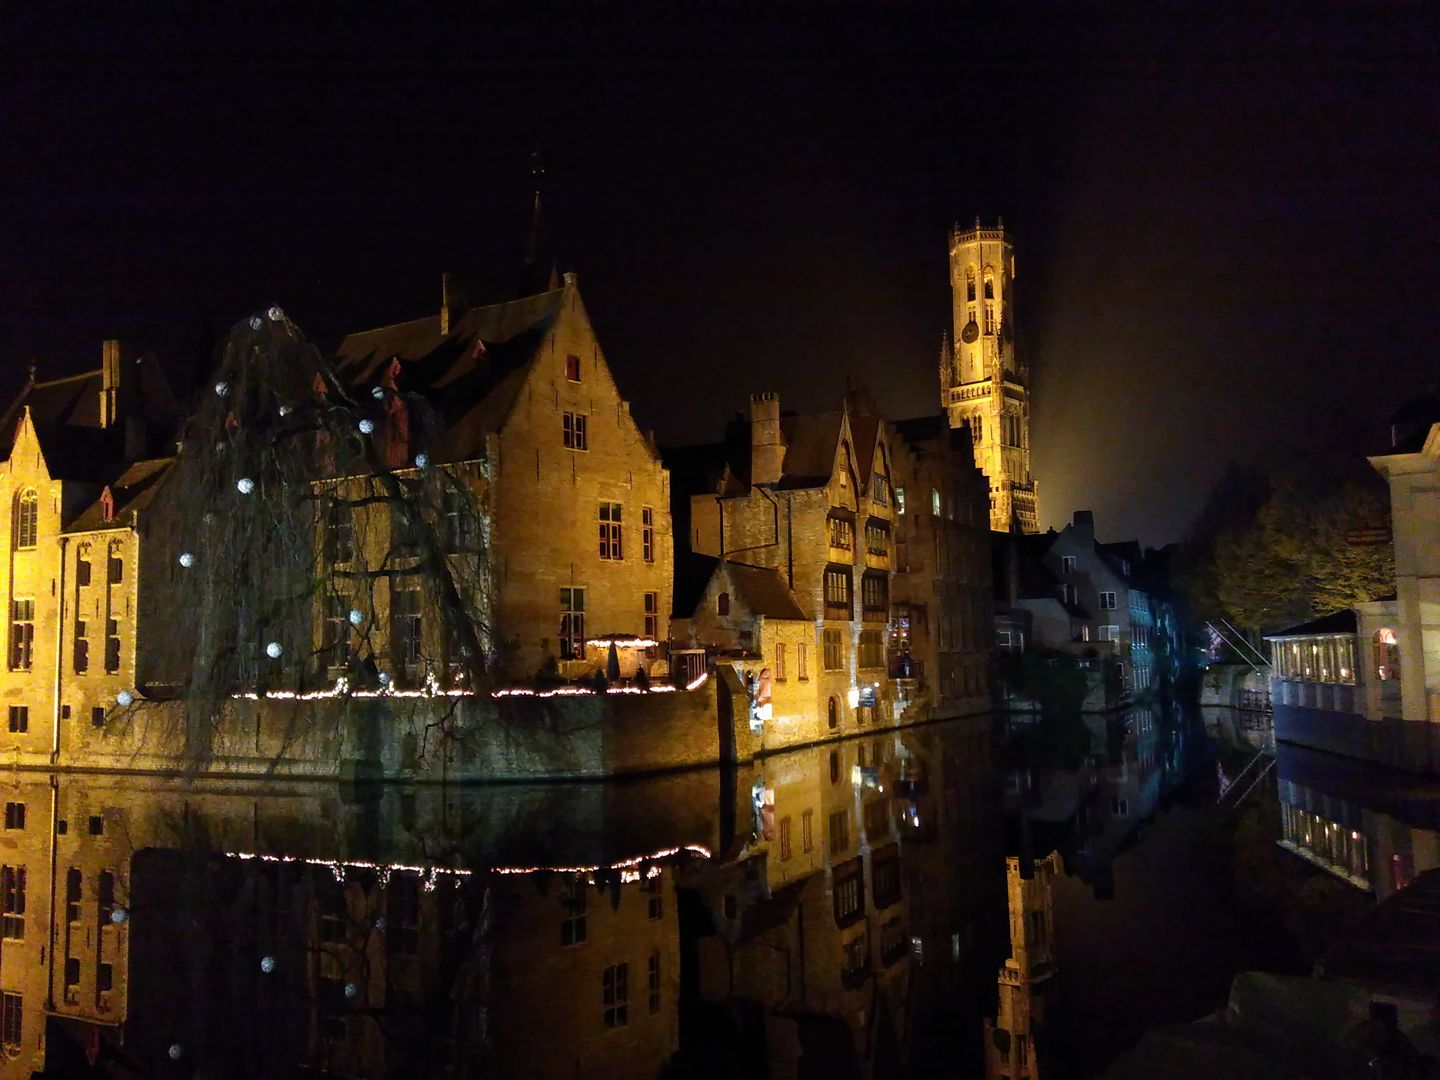
\includegraphics[scale=0.2]{bruges}
\end{figure}
\end{frame}


\section{Logical Relation}
%\subsection{Worlds}
\begin{frame}
  \frametitle{Worlds}
  \begin{overprint}
    \onslide<1>
    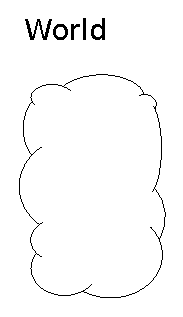
\includegraphics{World1.eps}
    \onslide<2>
    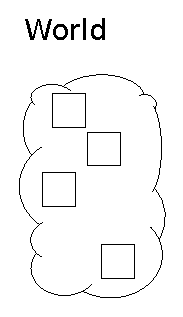
\includegraphics{World2.eps}
    \onslide<3>
    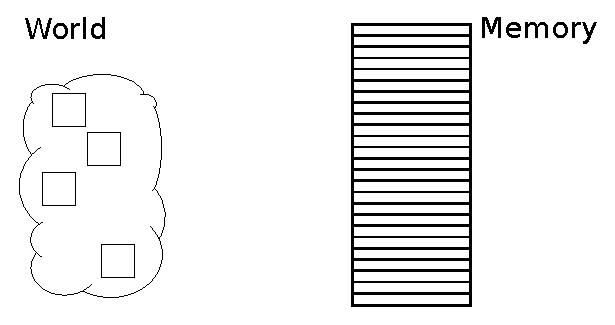
\includegraphics{World3.eps}
    \onslide<4>
    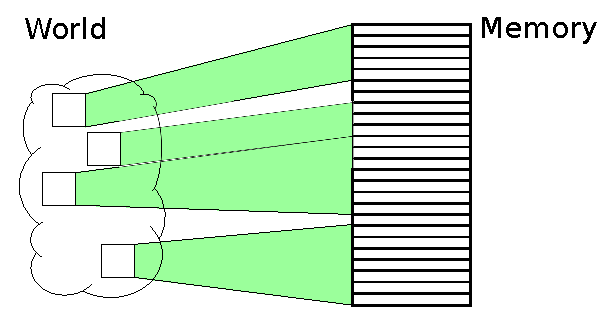
\includegraphics{World4.eps}
    \onslide<5>
    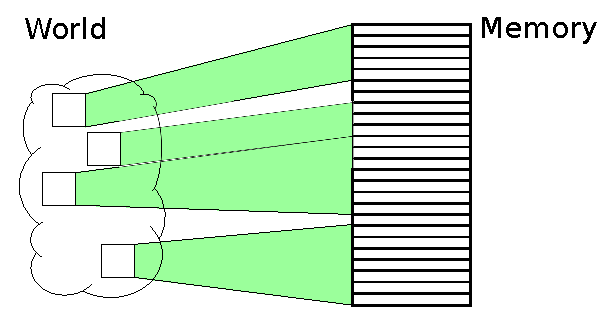
\includegraphics{World5.eps}
    \onslide<6>
    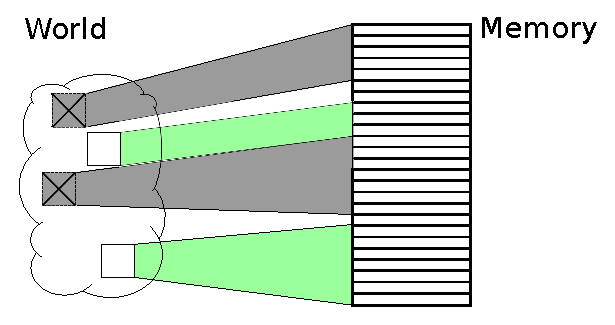
\includegraphics{World6.eps}
    \onslide<7>
    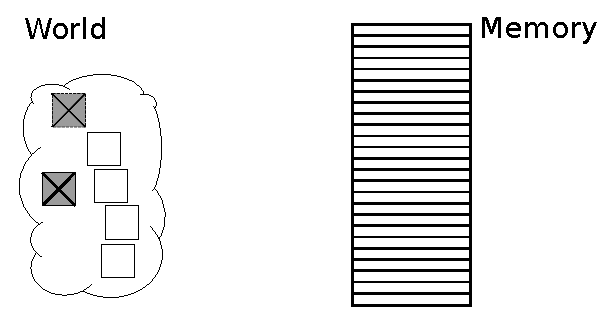
\includegraphics{World7.eps}
    \onslide<8>
    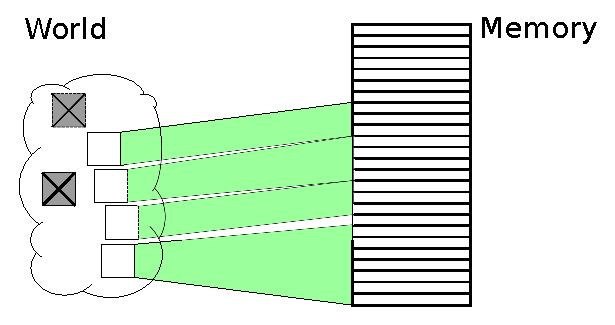
\includegraphics{World8.eps}
  \end{overprint}
\end{frame}
\begin{frame}
  \frametitle{Worlds}
  \begin{itemize}[<+->]
  \item $\Worlds : \nats \finparfun \Regions$
  \item Three kinds of regions:
    \begin{description}
    \item[permanent] Models parts of memory that global and local capabilities can govern.
    \item[temporary] Models parts of memory that only local capabilities can govern.
    \item[revoked] Masking of region.
    \end{description}

  \item Two future world relations
    \begin{description}
    \item[public]  Extensional  ($\futurewk$)
    \item[private] Extensional and temporary regions can be revoked! ($\futurestr$)
    \end{description}
  \end{itemize}
\end{frame}

\begin{frame}
  \frametitle{Regions}
  \begin{overprint}
    \onslide<1>
    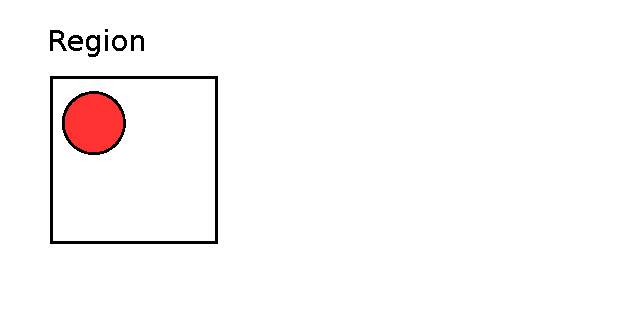
\includegraphics[trim=5px 5px 5px 5px]{region1.eps}
    \onslide<2>
    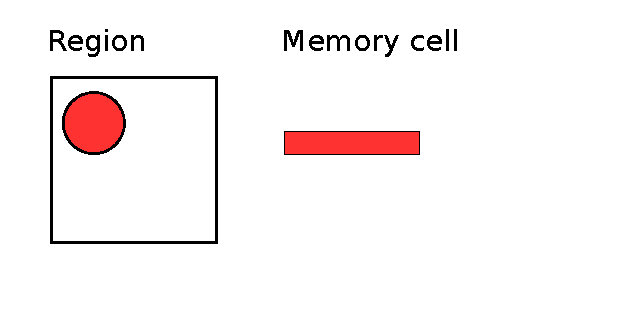
\includegraphics[trim=5px 5px 5px 5px]{region2.eps}
    \onslide<3>
    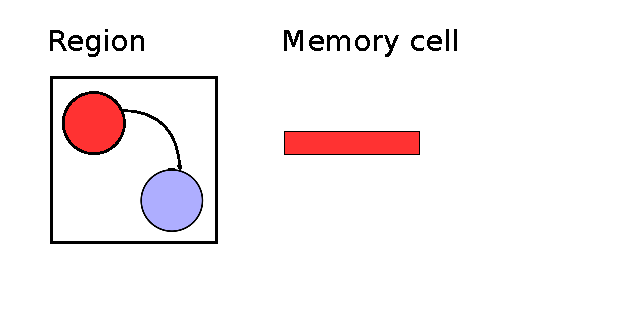
\includegraphics[trim=5px 5px 5px 5px]{region3.eps}
    \onslide<4>
    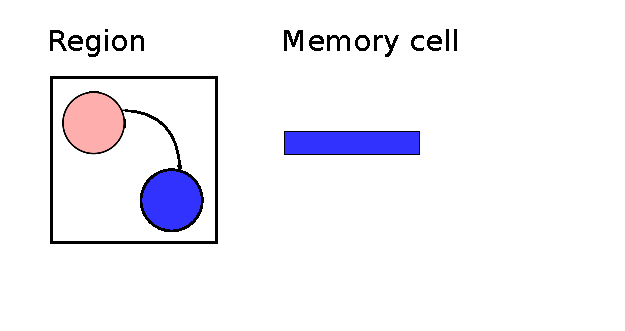
\includegraphics[trim=5px 5px 5px 5px]{region4.eps}
    \onslide<5>
    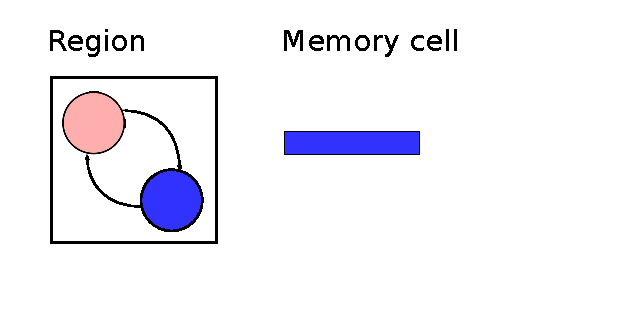
\includegraphics[trim=5px 5px 5px 5px]{region5.eps}
    \onslide<6>
    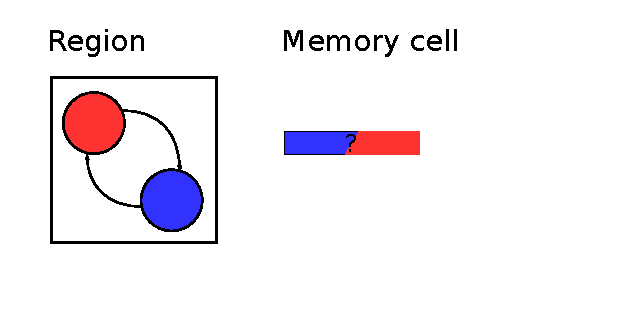
\includegraphics[trim=5px 5px 5px 5px]{region6.eps}
    \onslide<7>
    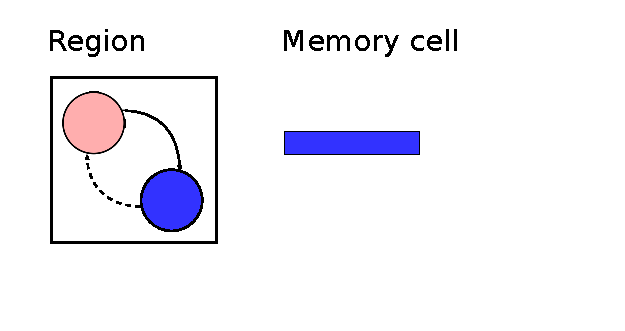
\includegraphics[trim=5px 5px 5px 5px]{region7.eps}
  \end{overprint}
\end{frame}

\begin{frame}
  \frametitle{Regions}
  \begin{itemize}[<+->]
  \item Regions are transition systems $(v,s,\phi_{\var{pub}},\phi,H)$
    \begin{itemize}
    \item $v$, view
    \item $s$, current state
    \item $\phi_{\var{pub}} : \States^2$, reflexive and transitive
    \item $\phi \supseteq \phi_{\var{pub}}$, reflexive and transitive
    \item $H : \States \fun \Worlds \monfun \UPred{\HeapSegments}$, state interpretation function
      \begin{itemize}
      \item if region permanent, then $H$ monotone w.r.t.\ $\futurestr$
      \item if region temporary, then $H$ monotone w.r.t.\ $\futurewk$
      \end{itemize}
    \end{itemize}
  \item Future Worlds
    \begin{itemize}
    \item In $\futurewk$, existing regions are allowed to make
      transitions in $\phi_{\var{pub}}$
  \item In $\futurestr$, existing regions are allowed to make transitions in $\phi$
  \end{itemize}
  \end{itemize}
\end{frame}



%\subsection{Predicates}
\begin{frame}
  \frametitle{Logical Relation}
  \begin{itemize}[<+->]
  \item Step indexed 
    \begin{itemize}
    \item but in the following, the steps are omitted.
    \end{itemize}
  \end{itemize}
\end{frame}
\begin{frame}
  \frametitle{Observation relation}
  \begin{itemize}
  \item Executable configurations that produce desired results.
  \end{itemize}
  \begin{align*}
    \observations : &  \Worlds \fun \UPred{\Regs \times \HeapSegments} \\
    \observations (W) \defeq & \{ (\reg,\hs) \mid
                               \begin{aligned}[t]
\onslide<2->{
                                 & \forall \ms_f, \heap'\ldotp \\
                                 & \quad(\reg,\hs \uplus \ms_f) \step (\halted,\heap')  \\}
\onslide<3->{
                                 & \qquad \Rightarrow
                                 \begin{aligned}[t]
                                   & \exists W' \futurestr W \ldotp\exists \hs_r, \hs' \ldotp\\
                                   & \quad \heap' = \hs' \uplus \hs_r \uplus \ms_f \land \\ 
                                   & \quad \heapSat[\hs']{}{W'} \}
                                 \end{aligned} }
                               \end{aligned}
  \end{align*}

\end{frame}

\begin{frame}
  \frametitle{Register-file relation}
  \begin{itemize}
  \item Register-files with ``well-behaved'' words.
  \item On jump, the contents of the register-file can be seen as the arguments.
  \end{itemize}
  \begin{align*}
    \stdrr : & \Worlds \monwkfun \UPred{\Regs} \\
    \stdrr(W) \defeq &
\onslide<2->{
                    \begin{aligned}[t]
                      \{ \reg \mid & \;\forall r \in \RegName \setminus \{\pcreg\} \ldotp \\
                      & \;\quad  \reg(r) \in \stdvr(W) \}
                    \end{aligned}
}
  \end{align*}
\end{frame}

\begin{frame}
  \begin{itemize}
  \item Words that produce admissable results when ``executed''.
  \end{itemize}
  \frametitle{Expression relation}
  \begin{align*}
    \stder : & \Worlds \fun \UPred{\Words} \\
    \stder(W) \defeq & \begin{aligned}[t]
\onslide<2->{
                      & \{ c \mid \forall \reg \in \stdrr(W) \ldotp \\
                      & \qquad  \forall \heapSat[\hs]{}{W} \ldotp \\}
\onslide<3->{
                      & \qquad \quad (\reg\update{\pcreg}{\pc},\hs) \in \observations(W) \} }
                    \end{aligned}
  \end{align*}
\end{frame}

\begin{frame}
  \frametitle{Value relation}
 $\stdvr$-relation
  \begin{itemize}[<+->]
  \item All integers (data) are in the $\stdvr$-relation
  \item For capabilities, define a condition for each kind of permission it grants
  \item Global capabilities
    \begin{itemize}
    \item Must respect $\futurestr$
    \item Authority only over memory segments governed by permanent region.
    \end{itemize}
  \item Local capabilities
    \begin{itemize}
      \item Must respect $\futurewk$
      \item Authority over memory segments governed by either permanent or temporary regions
    \end{itemize}
  \end{itemize}
\end{frame}




\begin{frame}
\frametitle{Read condition}
\begin{align*}
  & \readCond{}(\gl,W,\start,\addrend) =  \\
  & \quad \begin{aligned}[t]
    \{ (\start,\addrend) \mid & \;\exists r \in \var{localityReg}(g,W) \ldotp \\
    & \;\quad \exists [\start',\addrend'] \supseteq [\start,\addrend] \ldotp \\
    & \;\qquad W(r)\subset \iota_{\start',\addrend'}^\pwl \}
  \end{aligned}
\end{align*}
\onslide<2->
\[
  \iota_{\start,\addrend}^\pwl \defeq (\temp,1,=,=,H^\pwl_{\start,\addrend})
\]
\onslide<3->
\begin{align*}
  &H^\pwl : \Addrs^2 \fun \States \fun (\Worwk \monnefun \UPred{\HeapSegments})\\
  &H^\pwl_{\start,\addrend}\; s \; \hat{W} \defeq \left\{\hs \middle|
    \begin{aligned}
      &\dom(\hs) = [\start,\addrend] \land \\
      &\forall \addr \in [\start,\addrend] \ldotp \hs(\addr) \in \stdvr(\hat{W})
    \end{aligned}
        \right\}
\end{align*}

\end{frame}

\begin{frame}
  \frametitle{Write condition}
  \begin{align*}
    & \writeCond{}(\iota,\gl,W,\start,\addrend) =  \\
    & \quad \begin{aligned}[t]
      \{ (\start,\addrend) \mid & \;\exists r \in \var{localityReg}(g,W) \ldotp \\
      & \;\quad \exists [\start',\addrend'] \supseteq [\start,\addrend] \ldotp \\
      & \;\qquad W(r)\supset \iota_{\start',\addrend'} \}
    \end{aligned}
  \end{align*}
  \onslide<2->
  \[
    \iota_{\start,\addrend}^{\nwl} \defeq (\temp,1,=,=,H^\nwl_{start,\addrend})
  \]
  \onslide<3->
  \begin{align*}
    &H^\nwl : \Addrs^2 \fun \States \fun (\Worstr \monnefun \UPred{\HeapSegments})\\
    &H^\nwl_{\start,\addrend} \; s \;\hat{W} \defeq \left\{\hs \middle|
      \begin{aligned}
        &\dom(\hs) = [\start,\addrend] \land \\
        &\forall \addr \in [\start,\addrend] \ldotp \\
        &\quad \hs(\addr) \in \stdvr(\revokeTemp{\hat{W}})
      \end{aligned}
          \right\}
  \end{align*}
\end{frame}


\begin{frame}
\frametitle{Conditions on execution}
\begin{align*}
  \onslide<1->{
  & \execCond{}(\gl,W,\perm,\start,\addrend) = \\
  & \quad
    \begin{aligned}[t]
      \{ (\perm,\start,\addrend) \mid 
      & \forall W' \future W \ldotp\\
      & \quad  \forall a \in [\start,\addrend] \ldotp\\
      & \qquad ((\perm,\gl),\start,\addrend,\addr) \in \stder(W')\}
    \end{aligned}} \\
  & \\
  & \onslide<3->{\entryCond{}(\gl,W,\start,\addrend,\addr) = \\
  & \quad
    \begin{aligned}[t]
      \{ (\start,\addrend,\addr) \mid 
      & \forall W' \future W \ldotp\\
      & \quad ((\exec,\gl),\start,\addrend,\addr) \in \stder(W')\}
    \end{aligned}} \\ 
  & \\
  & \onslide<2->{\quad \text{where } \gl = \local \Rightarrow \future = \futurewk \\
  & \quad \text{and } \gl = \glob \Rightarrow \future = \futurestr}
\end{align*}
\end{frame}

\begin{frame}
  \frametitle{Value relation}
  \begin{align*}
    &\stdvr : \Worlds \monwkfun \UPred{\Words} \\
    &\stdvr(W) \defeq
      \begin{aligned}[t]
\onslide<2->{
        & \{ i \mid i \in \ints \} 
        \union \\}
\onslide<3->{
        & \{ \stdcap[(\noperm,\gl)]  \} 
        \union \\}
\onslide<4->{
        & \{ \stdcap[(\entry,\gl)] \mid \\
        & \quad \entryCond{}(\gl,W,\start,\addrend,\addr)\} 
        \union \\}
\onslide<5->{
        & \{ \stdcap[(\rwlx,\gl)] \mid \\
        & \quad \readCond{}(\gl,W,\start,\addrend) \land \\
        & \quad \writeCond{}(\iota^\pwl,\gl,W,\start,\addrend) \land\\
        & \quad \execCond{}(\gl,W,\rwlx,\start,\addrend) \} \union \\}
\onslide<6->{
        & \quad \dots
}
      \end{aligned}
  \end{align*}
\end{frame}

\begin{frame}
  \frametitle{Fundamental Theorem of Logical Relations (FTLR)}
  \begin{overprint}
\onslide<1-3>
  \begin{lemma}[FTLR] 
  For all $W \in \Worlds$ and $c \in Caps$,
  \[
    c \in \stder(W).
  \]
\end{lemma}
\onslide<2-3>{
  \begin{itemize}
  \item<2-> The $\pcreg$-register can be accessed like any other register
  \item<3> Capability must behave when used for read/write
  \end{itemize}
}
\onslide<4>
\begin{lemma}[FTLR] 
  For all $W \in \Worlds$, $\gl \in \Globals$, $\perm \in \Perms$, and $\start,\addrend,\addr \in \Addrs$, 

  if
  \[ 
    \perm = \exec\text{ and }\readCond{g,W,\start,\addrend},
  \]
  or
  \begin{align*}
    & \perm = \rwx \text{ and } \readCond{W,\start,\addrend} \\
    &\text{ and } \writeCond{\iota^\nwl,g,W,\start,\addrend}
  \end{align*}
  or
  \[
    \dots 
  \]
  then 
  \[
    (\perm, \start, \addrend, \addr) \in \stder(W).
  \]
\end{lemma}
\end{overprint}
\end{frame}

\begin{frame}
  \frametitle{The awkward example}
  \begin{itemize}[<+->]
  \item Using the logical relation, we can prove well-bracketedness for for the awkward example.
  \item The proof will have to wait for another time.
  \end{itemize}
\vspace{1cm}
  \usebox{\awkwardex}
\end{frame}

\begin{frame}
  \frametitle{Namur}
  \begin{figure}
    \centering
    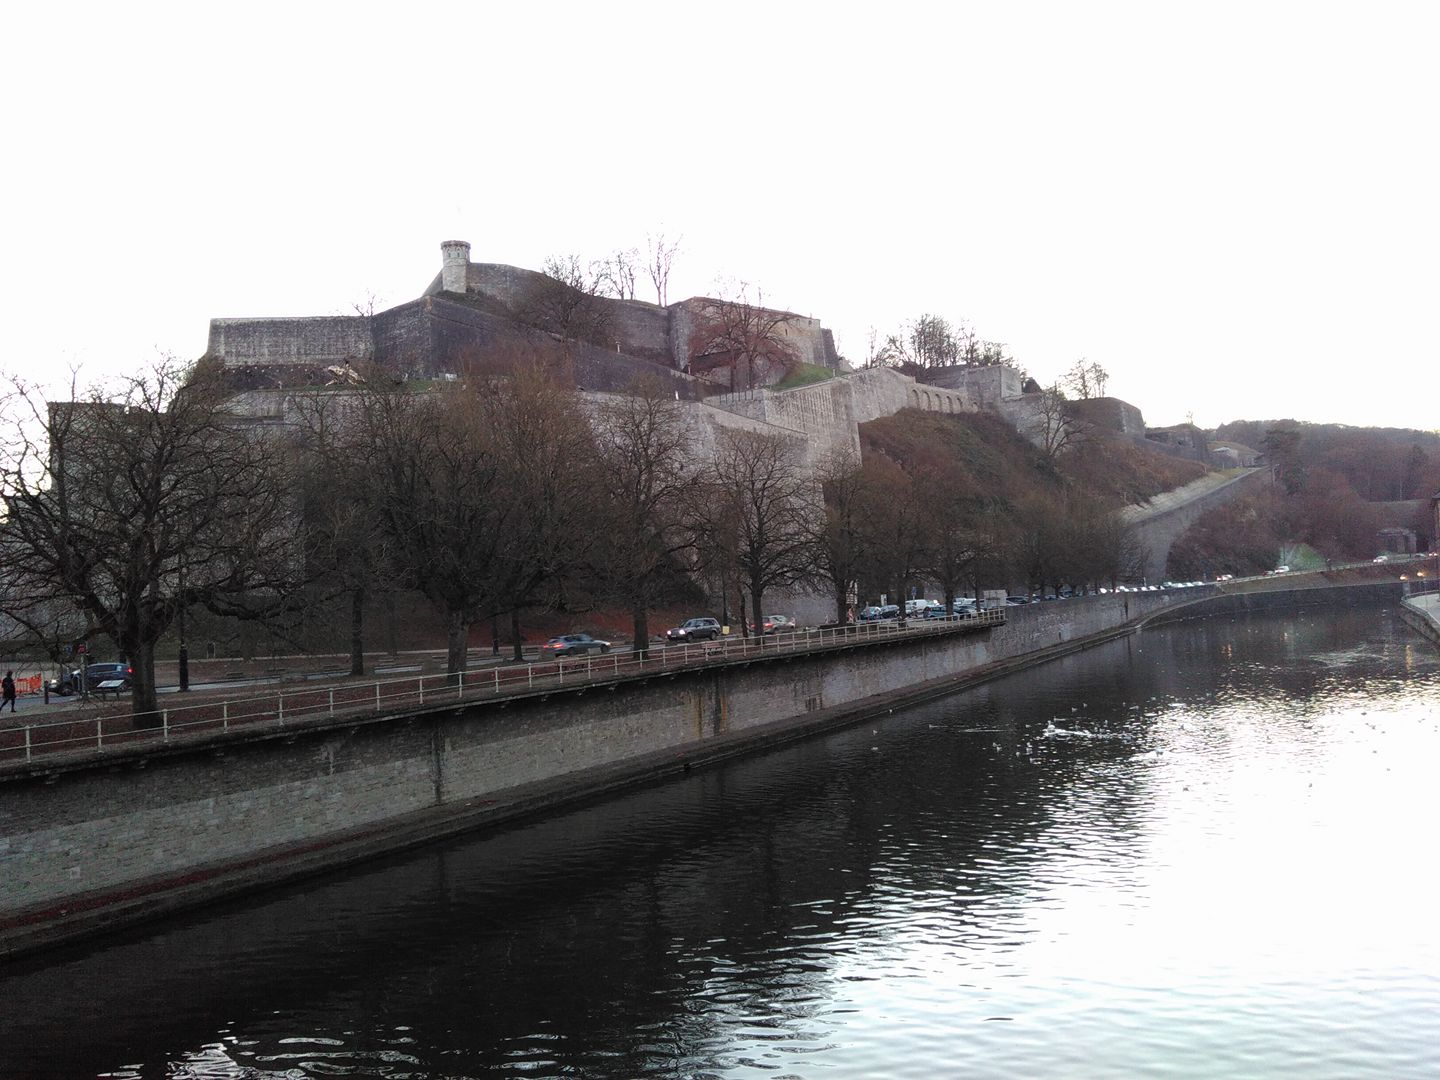
\includegraphics[scale=0.2]{nam}
\end{figure}
\end{frame}

\section{Conclusion}
\begin{frame}
  \frametitle{Conclusion}
  \begin{itemize}
  \item With a simple capability system and reasonable conventions, we can enforce well-bracketedness.
  \item Using known logical relation techniques, we can reason about programs for a simple capability machine.
  \end{itemize}
\end{frame}

\begin{frame}
  \frametitle{Questions?}
  \begin{itemize}
  \item<2-> Chocolates in the kitchen. 
  \end{itemize}
\end{frame}

\frame{
\frametitle{References}
  \bibliographystyle{plainnat}
  \bibliography{refs}
}


\end{document}

